Training the model with different sizes of latent dimensions yielded some different results, in different aspects of the task the model had. We can see how the training loss progressed through the epochs in Figure ~\ref{fig:cnn_loss}.\\

\begin{figure}[!ht]
  \centering
  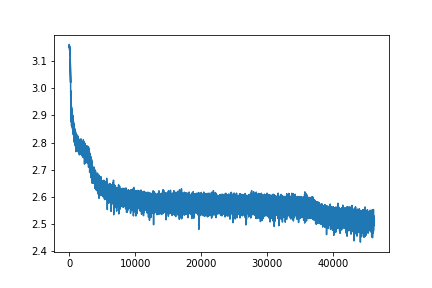
\includegraphics[width=0.4\linewidth]{latex/imgs/CNN_loss_latent_dimension_100.png}
  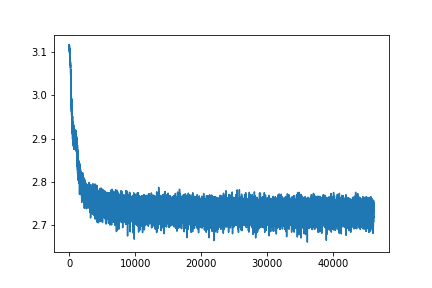
\includegraphics[width=0.4\linewidth]{latex/imgs/loss_latent_dimension_50.png}
  \caption{losses of the of cnn trained with latent dimension $4$x$100$(left) and $2$x$50$(right)}
  \label{fig:cnn_loss}
\end{figure}

\noindent
As can be seen on the graph (Figure ~\ref{fig:cnn_loss}), the one with a high latent dimension had a noticeably better loss, than the one with a lower latent dimension. Which makes good sense, since the model with a greater latent dimension has more data to use in the reconstruction. Since the loss was based on the model's ability to reconstruct the image; it is no surprise that the one with higher dimensionality reduction, had better reconstruction accuracy.

\begin{table}[!ht]
\centering
\begin{tabular}{|l|l|l|}
\hline
 latent\_dimension: & $4$x$100$  &  $2$x$50$ \\ \hline
min\_loss model     & 0.2039 & 0.1473 \\ \hline
fully trained model & 0.2058 & 0.1469 \\ \hline
\end{tabular}
\caption{reconstruction accuracy}
\end{table}

\noindent
It's important to note that the reconstruction accuracy is not representative of the models performance on the separation or the stability prediction tasks.\\

\noindent
Figures ~\ref{fig:plot_50} and ~\ref{fig:plot_100} show the structural plotting of the model's latent representation run through a TSNE dimensionality reduction. The model does find some separation between the different structural classes, but it does not seem to be nearly as clean as the LSTM results. As can be seen, both models find some separation between classes (C, B, G) with some overlap. The rest of the classes are mostly spread out between the groups. This result indicates that this model is not very good at finding much structural separation. \\

\begin{figure}[!ht]
  \centering
  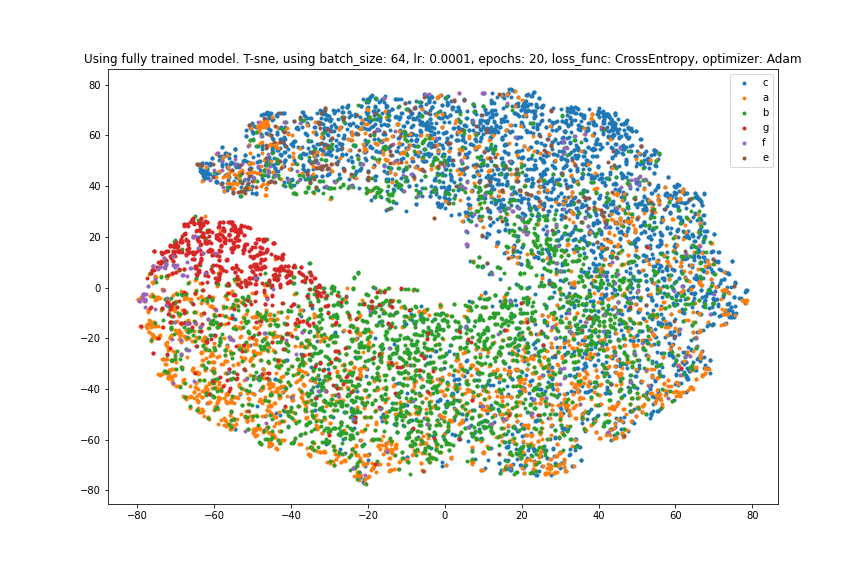
\includegraphics[width=0.4\linewidth]{latex/imgs/last_50.png}
  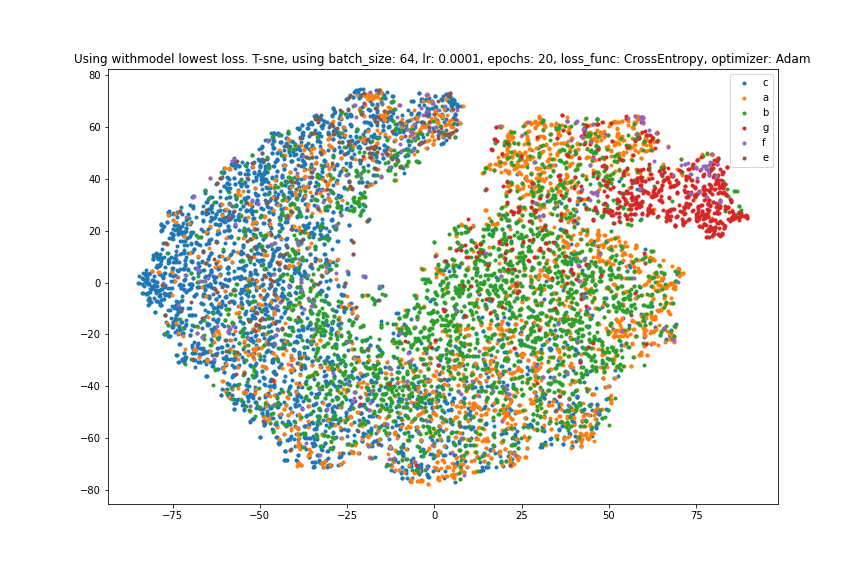
\includegraphics[width=0.4\linewidth]{latex/imgs/best_50.png}
  \caption{Plot showing secondary structure seperation with latent dimension $2$x$50$. Fully trained model(left), min loss model (left)}
  \label{fig:plot_50}
\end{figure}

\begin{figure}[!ht]
  \centering
  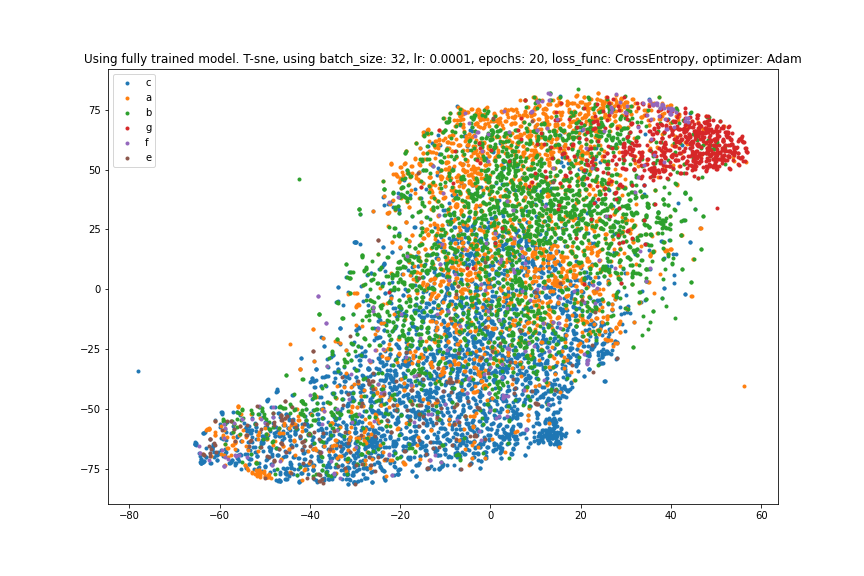
\includegraphics[width=0.4\linewidth]{latex/imgs/last_100.png}
  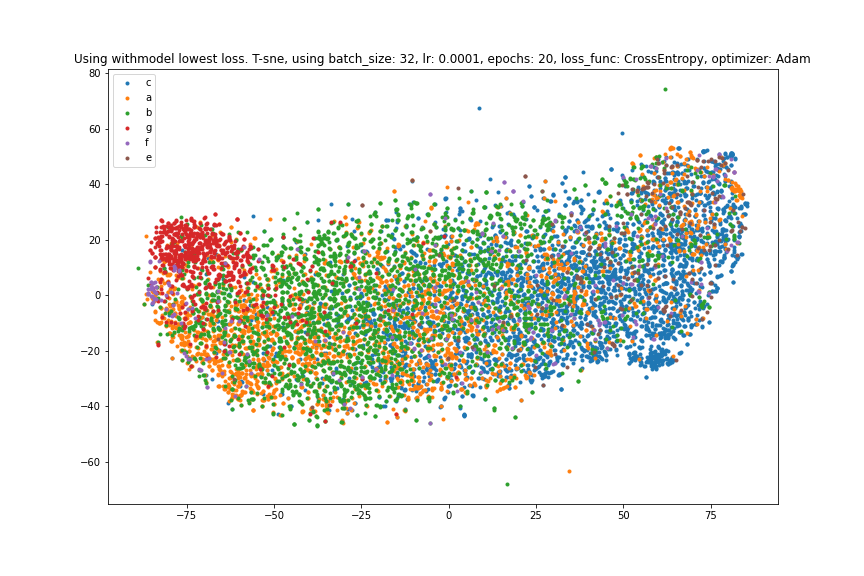
\includegraphics[width=0.4\linewidth]{latex/imgs/best_100.png}
  \caption{Plot showing secondary structure seperation with latent dimension $4$x$100$. Fully trained model(left), min loss model (left)}
  \label{fig:plot_100}
\end{figure}

\noindent
Figures ~\ref{fig:stab_100} and ~\ref{fig:stab_50}) show the resulting Spearman correlation data plots. With results

\begin{figure}[!ht]
  \centering
  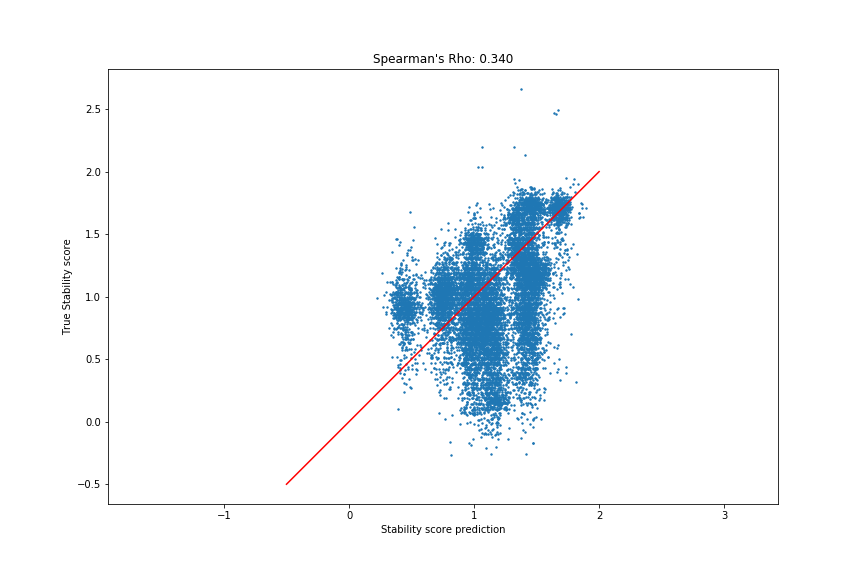
\includegraphics[width=0.4\linewidth]{latex/imgs/CNN_spearman_correlation_100_fully.png}
  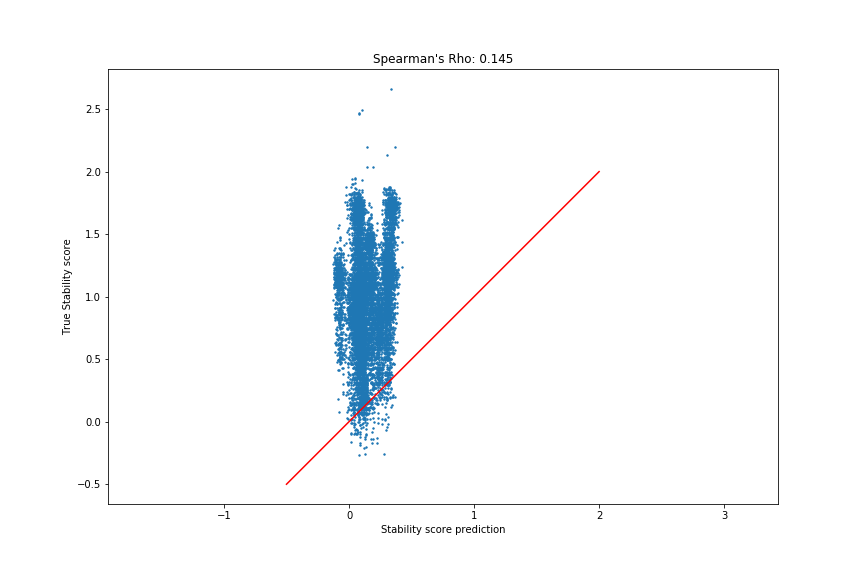
\includegraphics[width=0.4\linewidth]{latex/imgs/CNN_spearman_correlation_100_best.png}
  \caption{Graph showing the spearman correlation from model with latent dimension $4$x$100$. Fully trained model(left), min loss model (left)}
  \label{fig:stab_100}
\end{figure}

\begin{figure}[!ht]
  \centering
  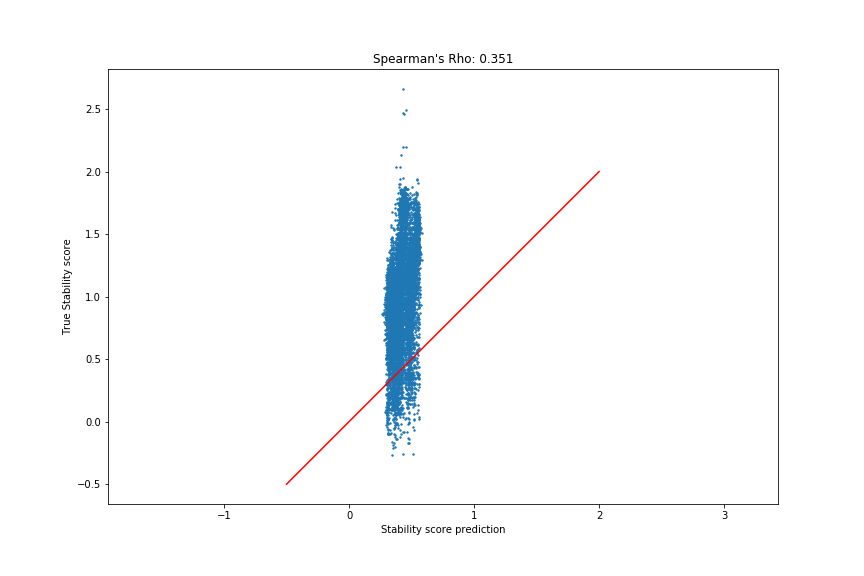
\includegraphics[width=0.4\linewidth]{latex/imgs/CNN_spearman_correlation_50_fully.png}
  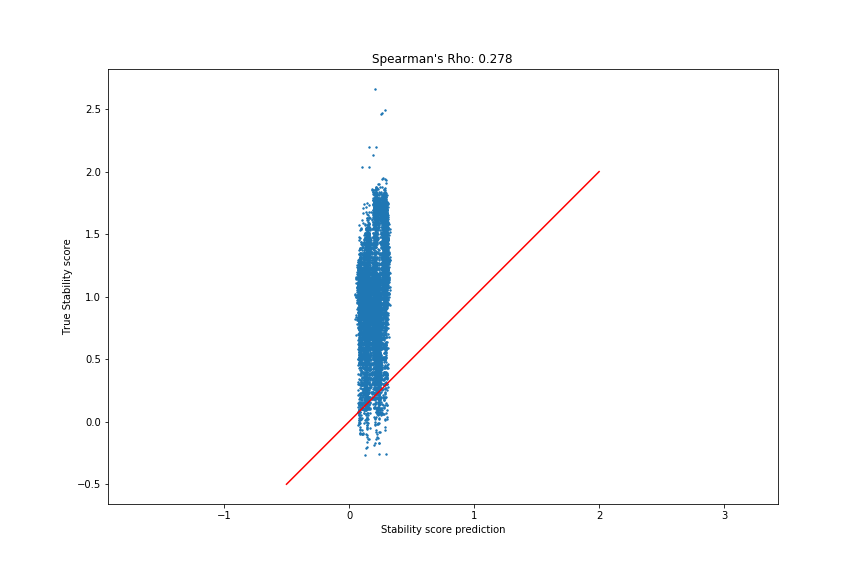
\includegraphics[width=0.4\linewidth]{latex/imgs/CNN_spearman_correlation_50_best.png}
  \caption{Graph showing the spearman correlation from model with latent dimension $2$x$50$. Fully trained model(left), min loss model (left)}
  \label{fig:stab_50}
\end{figure}

\noindent
It would seem that the model converges at about 0.3, which not especially great results since they are pretty far from the optimal results 1. Yet, it means that the model has learned some representation of the structure. \\

\noindent
In general in these experiments, the results from the minimum loss model, doesn't perform that different compared to the fully trained model.